\documentclass{article}
\usepackage[space]{ctex}
\usepackage{graphicx}
\usepackage{minted}
\usepackage{float}
\graphicspath{{pic/}}
\usepackage{hyperref}
\begin{document}
当安排日程时,我们首先会考虑是否有会议预订。但是如果需要为更重要的事情腾出时间,我们可能会取消某些次要的会议。

但是 RNN 并不能做到这样,为了添加一个新信息,它需要通过一个函数完全地转换当前的信息。因此信息是以整体为单位进行修改的,模型并没有考虑重要的和不重要的信息。

另一方面,LSTM 会通过乘法和加法等运算对信息进行局部的修改。因此通过 LSTM,信息流会选择性地通过单元状态,也就是说 LSTM 会选择性地记忆或遗忘某些特征。此外,特定单元状态下的信息共有三种不同的依赖性。

我们将用一些例子理解这一点,若我们特定股票的股价为例,那么当今股价取决于:

前几天的股票走势,如上升或下降等,即前面时间步的单元状态或记忆的信息;

前一天的收盘价,因为它与当天的开盘价有很大的关系,即前一时间步的隐藏单元状态或记忆的信息;

当天可能影响股票的因素,即当前 LSTM 单元的输入值或输入的新信息。

LSTM 另一个比较重要的特征是它的序列处理方式,LSTM 利用这种方式收集更多的信息与语境关系。下图展示了 LSTM 的这种序列式的处理方式:
\begin{figure}[H]
	\centering
	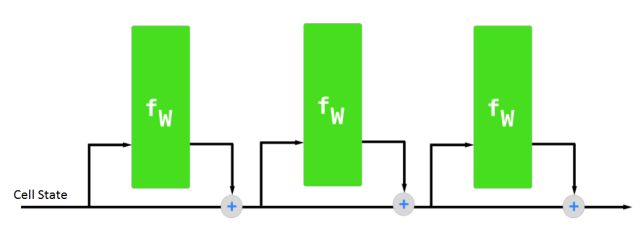
\includegraphics[scale=0.3]{1.png}
\end{figure}
虽然上图并没有表明详细和真实的 LSTM 架构,但它能给我们一个直观的理解。此外,正因为 LSTM 这种属性,它不会对整个信息进行统一的运算,而是稍微修改一些局部的信息。因此 LSTM 可以选择性地记住或遗忘一些事情,它也就有了「较长的短期记忆」。

\section{LSTM 架构}

通过了解新闻报道谋杀案的过程,我们可以类似地理解与可视化 LSTM 的运算过程。现在假设一条新闻是围绕许多事实、证据和证人所构建的,无论发生任何谋杀事件,我们都可以通过这三方面进行报道。

例如,若最初假设谋杀是通过给被害人下毒完成的,但尸检报告表明死亡原因是「对头部的影响」。那么作为新闻团队的一部分,我们很快就会「遗忘」前面的原因,后主要关注后面的原因而展开报道。

如果一个全新的嫌疑人进入了我们的视角,而该嫌疑人曾怨恨被害者,那么是否他有可能就是凶手?因此我们需要把他「输入」到我们的新闻中作进一步分析。

但是现在所有这些碎片信息都不够在主流媒体上进行报道,因此在一段时间后,我们需要总结这些信息并「输出」对应的结果给我们的读者。也许这个输出就表明并分析了到底谁才是概率最大的凶手。

下面,我们将详细介绍 LSTM 网络的架构:
\begin{figure}[H]
	\centering
	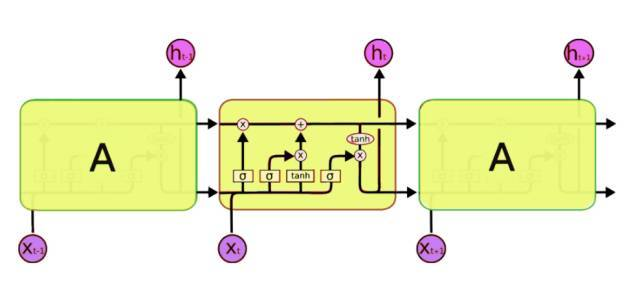
\includegraphics[scale=0.3]{2.jpg}
\end{figure}
这个架构和我们之间了解的简化版完全不同,但是本文将详细解释它。一个典型的 LSTM 网络由不同的单元或记忆块组成,即上图中我们看到的黄色矩形块。LSTM 单元一般会输出两种状态到下一个单元,即单元状态和隐藏状态。记忆块负责记忆各个隐藏状态或前面时间步的事件,这种记忆方式一般是通过三种门控机制实现,即输入门、遗忘门和输出门。
\section{遗忘门}
我们下面将采用以下语句作为文本预测问题的案例,首先假设该语句已经馈送到 LSTM 网络中。
\begin{quote}
	\emph{Bob is a nice person.Dan on the other hand is evil.}
\end{quote}
当模型遇到了「person」后面的第一个句号,遗忘门可能就会意识到下一个语句的语境可能会发生变化。因此语句的主语可能就需要遗忘,主语所处的位置也就空了出来。而当我们讨论到「Dan」时,前面空出来的主语位置就应该分配给「Dan」。遗忘前一语句的主语「Bob」的过程就由遗忘门控制。

\begin{figure}[H]
	\centering
	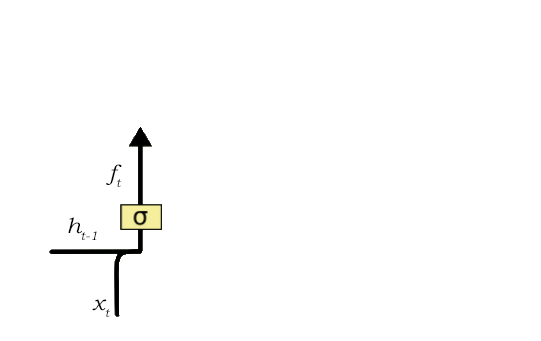
\includegraphics[scale=0.3]{3.png}
\end{figure}
遗忘门负责从单元状态中移除信息,LSTM 不需要这些信息来理解事物,这些不太重要的信息将通过滤波器运算而得到移除。这是优化 LSTM 性能所必须考虑的方面。

该遗忘门采取两个输入,即 $h_{t-1}$ 和 $x_t$。$h_{t-1}$ 为前一个单元的隐藏状态或输出状态,$x_t$ 为特定时间步的输入,即输入序列 x 的第 t 的元素。给定的输入向量与权重矩阵的乘积,再添加偏置项以输入 Sigmoid 函数。Sigmoid 函数将会输出一个向量,取值的范围为 0 到 1,其对应于单元状态中的每个数值。基本上,Sigmoid 函数决定保留哪些值和忘记哪些值。若单元状态取零这个特定值,那么遗忘门就要求单元状态完全忘记该信息。这个输出的 Sigmoid 函数向量最后会乘以单元状态。
\section{输入门}

下面我们使用另一个案例展示 LSTM 如何分析语句:
\begin{quote}
	\emph{Bob knows swimming.He told me over the phone that he had serverd the navy for 4 long years.}
\end{quote}
现在我们知道比较重要的信息是「Bob」知道游泳,且他在海军服役了四年。这可以添加到单元状态,因此这种添加新信息的过程就可以通过输入门完成。
\begin{figure}[H]
	\centering
	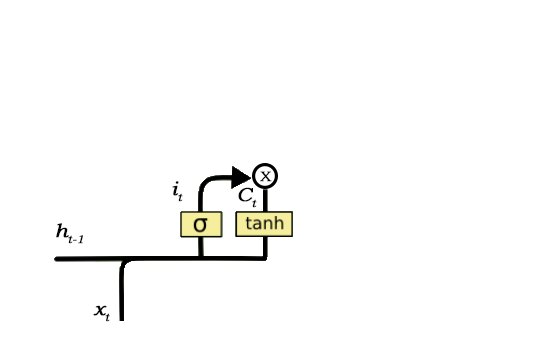
\includegraphics[scale=0.3]{4.png}
\end{figure}
\begin{itemize}
	\item     通过 Sigmoid 函数来调节需要添加到单元状态的值,这与遗忘门非常相似,它起到的作用就是作为一个滤波器过滤来自 $h_{t-1}$ 和 $x_t$ 的信息。

\item     创建一个包含所有可能值的向量,它可以被添加到单元状态中。该过程通过使用 tanh 函数实现,输出值为-1 到 1.

\item     将调节滤波器的值(Sigmoid 门控)乘以创建的向量(tanh 函数),然后将这些有用的信息添加到单元状态中。
\end{itemize}
在完成这三个步骤后,我们基本上确保了添加到单元状态的信息都是重要的,且不是冗余的。
\section{ 输出门}
\begin{quote}
	\emph{Bob fought single handedly with the enemy and died for his country.For his contributions brave .}
\end{quote}
在这一语句中,空格处可以有大量选择。但是我们知道空格之前的输入「brave」是一个修饰名词的形容词。因此,不管怎样,空格处存在一个很强的名词倾向。因此,Bob 可能是一个正确的输出。


从当前单元状态中选择有用信息并将其显示为输出的工作是通过输出门完成的。其结构如下:
\begin{figure}[H]
	\centering
	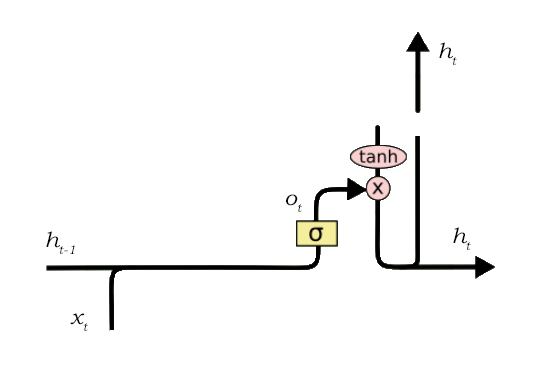
\includegraphics[scale=0.3]{5.png}
\end{figure}
输出门的功能可再次分为三个步骤:

\begin{enumerate}
\item 把 tanh 函数应用到单元状态之后创建一个向量,从而将值缩放在-1 到+1 之间。
\item 使用 $h_{t-1}$ 和 $x_t$ 的值生成一个过滤器,以便它可以调节需要从上述创建的向量中输出的值。这个过滤器再次使用一个 sigmoid 函数。
\item 将此调节过滤器的值乘以在步骤 1 中创建的向量,并将其作为输出发送出去,并发送到下个单元的隐藏态。
\end{enumerate}

上述实例中的过滤器将确保它减少除了「Bob」之外所有其他的值,因此过滤器需要建立在输入和隐藏态值上,并应用在单元状态向量上。
\section{LSTM 整体过程}

以上我们具体了解了 LSTM 的各个部分,但读者可能对 LSTM 的整体过程仍然不是太了解,下面我们简要地向读者介绍 LSTM 单元选择记忆或遗忘的具体处理流程。

以下是 LSTM 单元的详细结构,其中 Z 为输入部分,$Z_i$、$Z_o$ 和 $Z_f$ 分别为控制三个门的值,即它们会通过激活函数 f 对输入信息进行筛选。一般激活函数可以选择为 Sigmoid 函数,因为它的输出值为 0 到 1,即表示这三个门被打开的程度。
\begin{figure}[H]
	\centering
	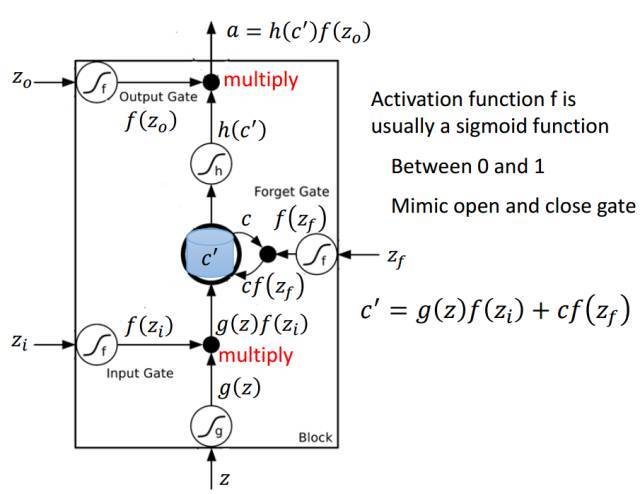
\includegraphics[scale=0.3]{6.jpg}
\end{figure}
若我们输入 Z,那么该输入向量通过激活函数得到的 g(Z) 和输入门 $f(Z_i)$ 的乘积 $g(Z)$ $f(Z_i )$ 就表示输入数据经筛选后所保留的信息。$Z_f$ 控制的遗忘门将控制以前记忆的信息到底需要保留多少,保留的记忆可以用方程 $c*f(z_f$)表示。以前保留的信息加上当前输入有意义的信息将会保留至下一个 LSTM 单元,即我们可以用 $c' = g(Z)f(Z_i) + cf(z_f)$ 表示更新的记忆,更新的记忆$ c'$ 也表示前面与当前所保留的全部有用信息。我们再取这一更新记忆的激活值 $h(c')$ 作为可能的输出,一般可以选择 tanh 激活函数。最后剩下的就是由 $Z_o$ 所控制的输出门,它决定当前记忆所激活的输出到底哪些是有用的。因此最终 LSTM 的输出就可以表示为 $a = h(c')f(Z_o)$。
\section{ 使用 LSTM 生成文本}

我们已经对 LSTM 的理论概念和功能有了足够了解。现在我们尝试建立一个模型,预测 Macbeth 原始文本之后的「n」的字符数量。绝大多数经典文本不再受版权保护,你可以在\href{https://www.gutenberg.org/}{这里}找到,更新的 TXT 版本可以在\href{https://s3-ap-south-1.amazonaws.com/av-blog-media/wp-content/uploads/2017/12/10165151/macbeth.txt}{这里}找到。

并非所有在单元状态运行的信息都适合在特定时间输出。我们将用一个实例进行展示:
我们使用 Keras,它是一个用于神经网络的高阶 API,并在 TensorFlow 或 Theano 之上工作。因此在进入代码之前,请确保你已安装运行正常的 Keras。好的,我们开始生成文本!

1. 首先导入必要的软件包:
\inputminted[firstline=1,firstnumber=1,lastline=7,linenos,breaklines,breakanywhere]{python}{lstm_predict.py}
2. 下载数据:
\inputminted[firstline=8,firstnumber=8,lastline=15,linenos,breaklines,breakanywhere]{python}{lstm_predict.py}
3. 将数据集中的单词映射为数值,然后分为50个序列,准备好数据。
\inputminted[firstline=16,firstnumber=16,lastline=37,linenos,breaklines,breakanywhere]{python}{lstm_predict.py}
4. 加速计算,当第一次训练完成后会保存模型和权重为my.h5文件。再次运行的时候直接载入,加速计算。
\inputminted[firstline=38,firstnumber=38,lastline=51,linenos,breaklines,breakanywhere]{python}{lstm_predict.py}
5. 预测验证模型
\inputminted[firstline=39,firstnumber=39,lastline=65,linenos,breaklines,breakanywhere]{python}{lstm_predict.py}
完整的源代码\href{https://github.com/bleedingfight/tfnote/blob/article/lstm_txt.py}{lstm\_predict.py}。

\end{document}

